% !TEX root = summary.tex
\documentclass[10pt,twocolumn, a4paper]{article}
\usepackage{amsmath, amssymb, amsthm, bm}
\usepackage{tikz}
\usetikzlibrary{decorations.pathreplacing, patterns}
\usepackage[utf8]{inputenc}
\usepackage[left=0.8cm,right=0.6cm,top=0.8cm,bottom=1.5cm]{geometry}
\usepackage{enumitem}
\setlist{nosep}
\usepackage{titlesec}
\titlespacing*{\section}{0pt}{0.5em}{0.2em}
\titlespacing*{\subsection}{0pt}{0.4em}{0.1em}
\titlespacing*{\subsubsection}{0pt}{0.3em}{0em}
\usepackage{parskip}
\setlength{\parskip}{0.3em}
\usepackage{nicefrac}


% Section formatting
%\titleformat{\section}{\large\bfseries\uppercase}{}{0em}{}[\titlerule]
%\titleformat{\subsection}{\bfseries}{}{0em}{}
%\titleformat{\subsubsection}{\small\bfseries}{}{0em}{}

\begin{document}

\twocolumn[
  \vspace{0cm}
  {\noindent\large\bfseries Summary of Structural Mechanics Modeling - Part 1 \hfill \small \today}
  \par\vspace{0.2em}\hrule\vspace{0.5em}
]

%\tableofcontents

\section{Tensor Calculus}

\subsection{Scalars, Vectors, and Tensors}
\begin{itemize}
    \item \textbf{Scalars (0th-order):} Magnitude only (e.g., density $\rho$, temperature $\theta$).
    \item \textbf{Vectors (1st-order):} Magnitude and direction. Decomposition: $\bm{v} = v_i \bm{e}_i$.
    \item \textbf{Second-order Tensors:} Linear transformations of vectors: $\bm{T}(\alpha \bm{u} + \beta \bm{v}) = \alpha \bm{T}\bm{u} + \beta \bm{T}\bm{v}$.
    \item \textbf{Action on Basis:} $\bm{T}\bm{e}_i = T_{ji} \bm{e}_j$ \\
    $\bm{T}\bm{e}_1 = T_{11} \bm{e}_1 + T_{21} \bm{e}_2 + T_{31} \bm{e}_3$ \\
    $\bm{T}\bm{e}_2 = T_{12} \bm{e}_1 + T_{22} \bm{e}_2 + T_{32} \bm{e}_3$ \\
    $\bm{T}\bm{e}_3 = T_{13} \bm{e}_1 + T_{23} \bm{e}_2 + T_{33} \bm{e}_3$ \\
    $[T] = \begin{bmatrix} T_{11} & T_{12} & T_{13} \\ T_{21} & T_{22} & T_{23} \\ T_{31} & T_{32} & T_{33} \end{bmatrix} 
    \leftrightarrow \bm{T}_{ij} = \bm{e}_i \cdot \bm{T} \bm{e}_j$
\end{itemize}

\subsection{Tensor Operations}
\begin{itemize}
    \item \textbf{Scalar/Inner Product (Vectors):} $\bm{u} \cdot \bm{v} = u_i v_i$.
    \item \textbf{Vector/Cross Product:} $\bm{u} \times \bm{v} = \epsilon_{ijk} u_i v_j \bm{e}_k$.
    \item \textbf{Dyadic Product:} $(\bm{a} \otimes \bm{b})\bm{v} = (\bm{b} \cdot \bm{v})\bm{a}$. Components: $[\bm{a} \otimes \bm{b}]_{ij} = a_i b_j$.
    \item \textbf{Tensor Inner Product / Double Contraction:} $\bm{S} : \bm{D} = \text{tr}(\bm{S}^T \bm{D}) = S_{ij} D_{ij}$.
    \item \textbf{Trace:} $\text{tr}(\bm{T}) = T_{ii}$. Invariant under coordinate transformation.
    \item \textbf{Determinant:} $\det \bm{T} = \epsilon_{ijk} T_{1i} T_{2j} T_{3k}$. Invariant.
    \item \textbf{Transpose:} $\bm{u} \cdot \bm{T}^T \bm{v} = \bm{v} \cdot \bm{T} \bm{u}$. Components: $[\bm{T}^T]_{ij} = T_{ji}$.
    \item \textbf{Decomposition:} Symmetric $\bm{E} = \frac{1}{2}(\bm{S} + \bm{S}^T)$, Skew-Symmetric $\bm{W} = \frac{1}{2}(\bm{S} - \bm{S}^T)$.
    \item \textbf{Symmetric/Skew:} $\bm{S}^T = \bm{S}$ (Sym), $\bm{S}^T = -\bm{S}$ (Skew).
    \item \textbf{Positive Definite:} $\bm{v} \cdot \bm{S}\bm{v} > 0 \quad \forall \bm{v} \neq \bm{0}$.
    \item \textbf{Invertible:} $\exists \bm{S}^{-1}$ s.t. $\bm{S}\bm{S}^{-1} = \bm{S}^{-1}\bm{S} = \bm{I}$. Commutation: $(\bm{S}^{-1})^T = (\bm{S}^T)^{-1} = \bm{S}^{-T}$.    
    \item \textbf{Orthogonal Tensor:} $\bm{Q}^T = \bm{Q}^{-1}$ i.e., $\bm{Q}\bm{Q}^T = \bm{I}$. $\det(\bm{Q}^T \bm{Q}) = (\det \bm{Q})^2 = 1 \implies \det \bm{Q} = \pm 1$.
    \item \textbf{Rotation/Proper Orthogonal:} Orthogonal $\bm{R}$ with $\det \bm{R} = 1$. Preserves handedness of frame.
\end{itemize}

\subsection{Coordinate Transformation / Change of Basis}
Change of basis from $\bm{e}_i$ to $\bm{e}'_i$: $\bm{e}'_i = Q_{mi} \bm{e}_m$ where $\bm{Q}$ is the rotation tensor.
\begin{itemize}
    \item \textbf{Transformation Matrix:} $Q_{ij} = \bm{e}_i \cdot \bm{e}'_j$ (Direction cosines). Note: indices vary by convention.
    \item \textbf{New Basis:} $\bm{e}'_i = \mathbf{Q} \bm{e}_i$ (if $\mathbf{Q}$ rotates basis).
    \item \textbf{Vector Components:} $[\bm{v}]_{\bm{e}'} = \bm{Q}^T [\bm{v}]_{\bm{e}}$. ($v'_i = Q_{ki} v_k$).
    \item \textbf{Tensor Components:} $[\bm{T}]_{\bm{e}'} = \bm{Q}^T [\bm{T}]_{\bm{e}} \bm{Q}$. ($T'_{ij} = Q_{ki} T_{kl} Q_{lj}$).
    \item \textbf{Invariants:} $I_1 = \text{tr}(\bm{T})$, $I_2, I_3 = \det(\bm{T})$ are same in both bases.
\end{itemize}

\subsection{Eigenvalues and Principal Invariants}
For symmetric tensors $\bm{S}$, eigenvalues $\lambda$ (Principal Values) and eigenvectors $\bm{n}$ satisfy $\bm{S}\bm{n} = \lambda \bm{n}$.
\textit{Note:} The largest and smallest principal values correspond to the maximum and minimum possible values of the diagonal entries (normal components) of the tensor in any coordinate system. \\
Characteristic equation: $\lambda^3 - I_1 \lambda^2 + I_2 \lambda - I_3 = 0$.

Principal Invariants:
\begin{align*}
    I_1(\bm{S}) &= \text{tr}(\bm{S}) = \lambda_1 + \lambda_2 + \lambda_3 \\
    I_2(\bm{S}) &= \frac{1}{2}[(\text{tr}\bm{S})^2 - \text{tr}(\bm{S}^2)] = \lambda_1\lambda_2 + \lambda_2\lambda_3 + \lambda_3\lambda_1 \\
    I_3(\bm{S}) &= \det \bm{S} = \lambda_1\lambda_2\lambda_3
\end{align*}
Spectral Decomposition: $\bm{S} = \sum_{i=1}^3 \lambda_i \bm{n}_i \otimes \bm{n}_i = \bm{Q} \bm{\Lambda} \bm{Q}^T$.
where $\bm{\Lambda} = \text{diag}(\lambda_i)$ and $\bm{Q} = [\bm{n}_1, \bm{n}_2, \bm{n}_3] $ orthogonal.

\subsection{Scalar, Vector and Tensor Fields}
\begin{itemize}
    \item \textbf{Differential:} $d\phi = \phi(\bm{x} + d\bm{x}) - \phi(\bm{x}) \approx \nabla \phi \cdot d\bm{x}$.
    \item \textbf{Gradient (Scalar):} $\nabla \phi = \frac{\partial \phi}{\partial x_i} \bm{e}_i = \phi_{,i}$.
    \item \textbf{Gradient (Vector):} $\nabla \bm{v} = \frac{\partial v_i}{\partial x_j} \bm{e}_i \otimes \bm{e}_j = v_{i,j}$.
    \item \textbf{Divergence (Vector):} $\nabla \cdot \bm{v} = \text{tr}(\nabla \bm{v}) = v_{i,i}$.
    \item \textbf{Divergence (Tensor):} $(\nabla \cdot \bm{S}) \cdot \bm{a} = \nabla \cdot (\bm{S}^T \bm{a})$. Components: $(\nabla \cdot \bm{S})_i = S_{ij,j}$.
    \item \textbf{Curl:} $\nabla \times \bm{v} = \epsilon_{ijk} v_{j,k} \bm{e}_i$.
    \item \textbf{Laplacian:} $\Delta \phi = \nabla \cdot (\nabla \phi) = \phi_{,ii}$.
\end{itemize}

\subsection{Integral Theorems}
\begin{itemize}
    \item \textbf{Divergence Theorem (Gauss):} $\int_{\partial B} \bm{v} \cdot \bm{n} \, dA = \int_B \nabla \cdot \bm{v} \, dV \leftrightarrow \int_{\partial B} v_i \hat{n}_i \, dA = \int_B v_{i,i} \, dV$.
    \item \textbf{Stokes' Theorem:} $\int_{\Gamma} (\nabla \times \bm{v}) \cdot \bm{n} \, dA = \int_C \bm{v} \cdot \bm{t} \, ds \leftrightarrow \int_{\Gamma} \epsilon_{ijk} v_{k,j} \hat{n}_i \, dA = \int_C v_i \hat{t}_i \, ds$.
\end{itemize}

\section{Fundamentals of Linear Elasticity}

\subsection{Kinematics}
\begin{itemize}
    \item \textbf{Motion:} $\bm{x} = \bm{\phi}(\bm{X}, t)$ resp. $\bm{X} = \bm{\phi^{-1}}(\bm{x}, t)$. Material coordinates $\bm{X}$, Spatial coordinates $\bm{x}$
    \item Satisfied if: $det(\nabla \phi) = det[\frac{\partial x_i}{\partial X_I}] > 0$.
    \item \textbf{Displacement:} $\bm{U}(\bm{X}, t) = \bm{x} - \bm{X}$. Spatial: $\bm{u}(\bm{x}, t) = \bm{x} - \bm{\phi}^{-1}(\bm{x}, t) = \bm{x} - \bm{X}$.
    \item \textbf{Velocity:} $\bm{V}(\bm{X}, t) = \frac{d\bm{x}}{dt} = \frac{d\bm{U}}{dt} = \frac{\partial \bm{U}}{\partial t} = \frac{\partial \bm{\phi}}{\partial t} \big|_{\bm{X}}$.
    \item \textbf{Acceleration:} $\bm{A}(\bm{X}, t) = \frac{\partial^2 \bm{\phi}}{\partial t^2}$. Spatial: $\bm{a}(\bm{x}, t) = \frac{\partial \bm{v}}{\partial t} + (\nabla \bm{v})\bm{v}$ (Material derivative).
    \item \textbf{Material Derivative:} $\frac{D (\cdot)}{Dt} = \frac{\partial (\cdot)}{\partial t} + \bm{v} \cdot \nabla (\cdot) = \frac{\partial (\cdot)}{\partial t} + \frac{\partial(\cdot)}{\partial x_i} v_i$.
\end{itemize}

\subsection{Deformation Gradient and Finite Strain}
\begin{itemize}
    \item \textbf{Deformation Gradient:} $\bm{F} = \frac{\partial \bm{x}}{\partial \bm{X}} = \nabla_{\bm{X}} \bm{\phi}$. Components $F_{ij} = \frac{\partial x_i}{\partial X_j} = \frac{\partial \phi_i}{\partial X_j} = x_{i,j} = \begin{bmatrix} \frac{\partial x_1}{\partial X_1} & \frac{\partial x_1}{\partial X_2} & \frac{\partial x_1}{\partial X_3} \\ \frac{\partial x_2}{\partial X_1} & \frac{\partial x_2}{\partial X_2} & \frac{\partial x_2}{\partial X_3} \\ \frac{\partial x_3}{\partial X_1} & \frac{\partial x_3}{\partial X_2} & \frac{\partial x_3}{\partial X_3} \end{bmatrix}$.
    \item \textbf{Jacobian:} $J = \det \bm{F} > 0$. Volume change: $dv = J dV = \det \bm{F} dV$. Incompressible/Isochoric if $J = 1$.
    \item \textbf{Length Change:} $(dx)^2 - (dX)^2 = 2d\bm{X} \cdot \bm{E} d\bm{X} = 2d\bm{x} \cdot \bm{e} d\bm{x}$.
    \item Howto get strain $\epsilon_{ij}$: 1) $u_1 = x_1 - X_1, u_2 = x_2 - X_2, u_3 = x_3 - X_3$ 2) $\nabla \bm{u} = u_{i,j} $ 3) $\epsilon_{ij} = \frac{1}{2}(\nabla \bm{u} + \nabla \bm{u}^T)$
    \item \textbf{Right Cauchy-Green Tensor:} $\bm{C} = \bm{F}^T \bm{F}$ ($C_{IJ} = F_{kI} F_{kJ}$). 
    \item \textbf{Green-Lagrange Strain:} $\bm{E} = \frac{1}{2}(\bm{C} - \bm{I})$. 
    \item \textbf{Left Cauchy-Green Tensor:} $\bm{b} = \bm{F} \bm{F}^T$ ($b_{ij} = F_{iK} F_{jK}$). Inverse: $\bm{b}^{-1} = \bm{F}^{-T} \bm{F}^{-1}$.
    \item \textbf{Euler-Almansi Strain:} $\bm{e} = \frac{1}{2}(\bm{I} - \bm{b}^{-1})$.
    \item \textbf{Finite Strain: } $\bm{\varepsilon} = \frac{1}{2}(\bm{F} + \bm{F^T}) - \bm{I}$. 
\end{itemize}

\subsection{Mapping and Fiber Deformation}
\begin{itemize}
    \item \textbf{Stretch Ratio $\lambda$ in direction $\bm{N}$:}
    \begin{enumerate}
        \item Compute $\bm{F} = \frac{\partial x_i}{\partial X_I}$.
        \item Deformed segment: $d\bm{x} = \bm{F} (dX \bm{N})$.
        \item $\lambda = \frac{\|d\bm{x}\|}{\|d\bm{X}\|} = \sqrt{\bm{N} \cdot \bm{C} \bm{N}}$.
    \end{enumerate}
    \item \textbf{Angle $\theta$ between deformed fibers ($\bm{N}_1, \bm{N}_2$):}
    \begin{enumerate}
        \item Compute deformed vectors: $d\bm{x}^{(1)} = \bm{F} d\bm{X}^{(1)}$, $d\bm{x}^{(2)} = \bm{F} d\bm{X}^{(2)}$.
        \item $\cos \theta = \frac{d\bm{x}^{(1)} \cdot d\bm{x}^{(2)}}{\|d\bm{x}^{(1)}\| \|d\bm{x}^{(2)}\|} = \frac{\bm{N}_1 \cdot \bm{C} \bm{N}_2}{\lambda_1 \lambda_2}$.
    \end{enumerate}
\end{itemize}

\subsection{Infinitesimal Strain $\bm{\varepsilon}_{ij}$}
Under assumption of small displacement gradients ($||\nabla \bm{u}|| \ll 1$): $\bm{E} \approx \bm{e} \approx \bm{\varepsilon}$. $\boxed{\bm{\varepsilon} = \nicefrac{1}{2}\;(\nabla\bm{u}+\nabla\bm{u}^T) \leftrightarrow\varepsilon_{ij}=\nicefrac{1}{2}\;(u_{i,j}+u_{j,i})}$
\begin{itemize}
    \item \textbf{Displacement Fields:}
    \begin{itemize}
        \item \textit{Infinitesimal Rigid Displacement:} $\bm{u}(\bm{x}) = \bm{u}_0 + \bm{W}(\bm{x} - \bm{x}_0)$ where $\bm{W}$ is skew-symmetric.
        \item \textit{Homogeneous Displacement:} $\bm{u}(\bm{x}) = \bm{u}_0 + \bm{A}(\bm{x} - \bm{x}_0)$ where $\bm{A}$ is a constant tensor.
    \end{itemize}
    \item \textbf{Normal Strains (Geometric Meaning):}
    Consider element $d\bm{X} = dS \bm{n}$. Deformed length $ds$.
    $$ \frac{ds - dS}{dS} = \bm{n} \cdot \bm{\varepsilon} \bm{n} = \varepsilon_{nn} $$
    $\varepsilon_{11}, \varepsilon_{22}, \varepsilon_{33}$ are unit elongations in $x_1, x_2, x_3$ directions.
    \item \textbf{Shear Strains (Geometric Meaning):}
    Consider perpendicular elements $d\bm{X}^{(1)} = dS_1 \bm{m}, d\bm{X}^{(2)} = dS_2 \bm{n}$ ($\bm{m} \cdot \bm{n} = 0$).
    Let $\theta$ be the angle between deformed elements. Decrease in angle $\gamma = \frac{\pi}{2} - \theta$. By $d\bm{x}^{(1)}\cdot d\bm{x}^{(2)} = ds_1ds_2cos\phi = 2dS_1dS_2\varepsilon_{mn}$:
    $$ \gamma = 2\varepsilon_{mn} = 2(\bm{m} \cdot \bm{\varepsilon} \bm{n}) $$
    $2\varepsilon_{ij} (i \neq j)$ is the decrease in angle between elements initially in $x_i$ and $x_j$ directions (Engineering Shear Strain).
    \item \textbf{Volume Change:} $e = \text{tr}(\bm{\varepsilon}) = \varepsilon_{kk} \approx \frac{dv - dV}{dV}$.
    \item \textbf{Compression: } Only if $\exists \,eigenvalue < 0 \text{ of } \varepsilon_{ij}$. 
    \item \textbf{Find deformation}: \\
    A) Given $\bm{x}$ as function of $\bm{X}$ and $d\bm{X^{(;)}}$ of $dS_k$. \\
    B) Find deformed elements: 
    1) $F_{ij} = \frac{\partial x_i}{\partial X_j} = \dots$ 
    2) $d \bm{x}^{(k)} = \bm{F}\,d\bm{X^{k}} = \bm{F}\,(dS_k\dots)$ \\
    C) Find stretches: $\frac{ds_k}{dS_k} = \frac{||d\bm{x}||}{dS_k}$ or their length changes $ds_k$: $(ds_k)^2 = d\bm{X}_k^T \bm{C} d\bm{X}_k$ and their change of angle: $ds_1 ds_2cos\phi = d\bm{X}^T_1 \bm{C} d\bm{X}_2 \rightarrow \text{change is: } \frac{\pi}{2}-\phi$.
    \textit{Note: Cauchy-Green $\bm{C}$ either $\bm{F}^T\bm{F}$ (Green-Lagrange Strain E) or $\bm{F}+\bm{F}^T$ (Finite Strain)}.
\end{itemize}

\subsection{Compatibility Conditions (Saint-Venant)}
Ensure integrability of strain field to displacement field. Necessary if strains are given.
\textbf{Note:} If $\varepsilon_{ij}$ are linear functions of coordinates, conditions are automatically satisfied. 

Short one-liner: $\varepsilon_{ij,kl} + \varepsilon_{kl,ij} - \varepsilon_{ik,jl} - \varepsilon_{jl,ik} = 0$

or 6 equations:
\begin{align*}    
    &\frac{\partial^2 \varepsilon_{11}}{\partial x_2^2} + \frac{\partial^2 \varepsilon_{22}}{\partial x_1^2} = 2 \frac{\partial^2 \varepsilon_{12}}{\partial x_1 \partial x_2} \\
    &\frac{\partial^2 \varepsilon_{22}}{\partial x_3^2} + \frac{\partial^2 \varepsilon_{33}}{\partial x_2^2} = 2 \frac{\partial^2 \varepsilon_{23}}{\partial x_2 \partial x_3} \\
    &\frac{\partial^2 \varepsilon_{33}}{\partial x_1^2} + \frac{\partial^2 \varepsilon_{11}}{\partial x_3^2} = 2 \frac{\partial^2 \varepsilon_{13}}{\partial x_3 \partial x_1} \\
    &\frac{\partial^2 \varepsilon_{11}}{\partial x_2 \partial x_3} = \frac{\partial}{\partial x_1} \left( -\frac{\partial \varepsilon_{23}}{\partial x_1} + \frac{\partial \varepsilon_{13}}{\partial x_2} + \frac{\partial \varepsilon_{12}}{\partial x_3} \right) \\
    &\frac{\partial^2 \varepsilon_{22}}{\partial x_3 \partial x_1} = \frac{\partial}{\partial x_2} \left( \frac{\partial \varepsilon_{23}}{\partial x_1} - \frac{\partial \varepsilon_{13}}{\partial x_2} + \frac{\partial \varepsilon_{12}}{\partial x_3} \right) \\
    &\frac{\partial^2 \varepsilon_{33}}{\partial x_1 \partial x_2} = \frac{\partial}{\partial x_3} \left( \frac{\partial \varepsilon_{23}}{\partial x_1} + \frac{\partial \varepsilon_{13}}{\partial x_2} - \frac{\partial \varepsilon_{12}}{\partial x_3} \right)
\end{align*}

\newpage
\subsection{Motion and Equilibrium (Conservation Laws)}
\begin{itemize}
    \item \textbf{Cauchy Stress Principle:}\\
    material continuous distributed, forces can develop anywhere \\
    forces = body forces + surface forces\\
    plane surfaces (no curvatures)
    \item \textbf{Traction vector:} $\bm{t}_{\bm{n}} = \lim_{\Delta A \to 0} \frac{\Delta \bm{F}}{\Delta A} \rightarrow \boxed{\bm{t}_{\bm{n}} = \bm{\sigma} \bm{n}}$. \\
    Normal component $t_n = \bm{n}\cdot\bm{t_n}$; $t_n > 0$ tensile, $t_n < 0$ compressive. 
    Shearing component $t_s = \sqrt{||\bm{\sigma}\bm{n}||^2-(\bm{n\cdot\sigma n})^2}$. \\
    \textit{Note:} $\bm{t}_{-\bm{n}} = \lim_{\Delta A \to 0} \frac{-\Delta \bm{F}}{\Delta A} = -\bm{t}_{\bm{n}}$.
    \textit{Howto Max shearing stress:} Find eigenvectors $\lambda_i$, then $\frac{\lambda_max-\lambda_min}{2}$ acting on plane $\hat{v}_{\lambda_{max}}, \hat{v}_{\lambda_{min}}   $. 
    \item \textbf{Resulting Force and Momentum: } $\bm{F}=\int_A \bm{t_n} dA$. Get $\bm{M}$ by TM1 or $\bm{M}\int_A \bm{x} \times \bm{t_n}dA$. 
    \item \textbf{Cauchy Stress Tensor $\bm{\sigma}$:} Symmetric $\bm{\sigma} = \bm{\sigma}^T$ \\
    \textbf{Stress Vectors:} $\bm{t}_{\bm{e}_j} = \bm{\sigma} \bm{e}_j$ (Acting on plane with normal $\bm{e}_j$). \\
    Decomposition: $\bm{t}_{\bm{e}_1} = \sigma_{11} \bm{e}_1 + \sigma_{21} \bm{e}_2 + \sigma_{31} \bm{e}_3$. \\
    \textbf{Indices:} $\sigma_{ij}$: $i$ is the direction, $j$ is the plane (normal). \\
    \textbf{Normal Stress:} $\sigma_{ii}$ (tensile $> 0$, compressive $< 0$). \\
    \textbf{Shearing} (Tangential) \textbf{stresses:} $\sigma_{ij}$ with $i \neq j$. Resultant shear magnitude on plane $\bm{e}_1$: $|\tau_1| = \sqrt{\sigma_{21}^2 + \sigma_{31}^2}$.
    \item \textbf{Angular Momentum:} Leads to symmetry $\sigma_{ij} = \sigma_{ji}$.
\end{itemize}

\begin{center}
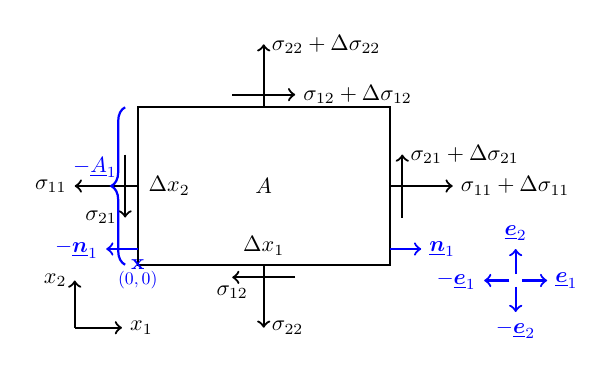
\begin{tikzpicture}[scale=0.8, every node/.style={scale=0.8}]
    % Coordinates and Recangle
    \draw[thick] (0,0) rectangle (4,2.5);
    \node at (2,1.25) {$A$};
    \node at (2,0.3) {$\Delta x_1$};
    \node at (0.5,1.25) {$\Delta x_2$};
    
    % Stress vectors
    % Left Face (-e1)
    \draw[thick, ->] (0,1.25) -- (-1,1.25) node[left] {$\sigma_{11}$};
    \draw[thick, ->] (-0.2,1.75) -- (-0.2,0.75) node[left] {$\sigma_{21}$};
    
    % Right Face (+e1)
    \draw[thick, ->] (4,1.25) -- (5,1.25) node[right] {$\sigma_{11} + \Delta \sigma_{11}$};
    \draw[thick, ->] (4.2,0.75) -- (4.2,1.75) node[right] {$\sigma_{21} + \Delta \sigma_{21}$};
    
    % Bottom Face (-e2)
    \draw[thick, ->] (2,0) -- (2,-1) node[right] {$\sigma_{22}$};
    \draw[thick, ->] (2.5,-0.2) -- (1.5,-0.2) node[below] {$\sigma_{12}$};

    % Top Face (+e2)
    \draw[thick, ->] (2,2.5) -- (2,3.5) node[right] {$\sigma_{22} + \Delta \sigma_{22}$};
    \draw[thick, ->] (1.5,2.7) -- (2.5,2.7) node[right] {$\sigma_{12} + \Delta \sigma_{12}$};

    % Coordinate System (x1, x2)
    \begin{scope}[shift={(-0.25,-0.25)},scale=0.75]
        \draw[thick, ->] (-1,-1) -- (0,-1) node[right] {$x_1$};
        \draw[thick, ->] (-1,-1) -- (-1,0) node[left] {$x_2$};
    \end{scope}
    % Coordinate Frame (Basis vectors) bottom right
    \begin{scope}[shift={(6,-0.25)}]
        \draw[thick, blue, ->] (0.1,0) -- (0.5,0) node[right] {$\bm{\underline{e}}_1$};
        \draw[thick, blue, ->] (0,0.1) -- (0,0.5) node[above] {$\bm{\underline{e}}_2$};
        \draw[thick, blue, ->] (-0.1,0) -- (-0.5,0) node[left] {$-\bm{\underline{e}}_1$};
        \draw[thick, blue, ->] (0,-0.1) -- (0,-0.5) node[below] {$-\bm{\underline{e}}_2$};
    \end{scope}

    % Blue annotations (A1, (0,0), axis at bottom right) - simplified
    \node[blue] at (0,0) {\textbf{x}};
    \node[blue] at (0,0) [midway, below] {$(0,0)$};
    \draw[blue, thick, decorate, decoration={brace,amplitude=5pt}] (-0.2,0) -- (-0.2,2.5) node[midway, above left] {$-\underline{A}_1$};

    % Normal vectors
    \draw[thick, blue, ->] (0,0.25) -- (-0.5,0.25) node[left] {$-\bm{\underline{n}}_1$};
    \draw[thick, blue, ->] (4,0.25) -- (4.5,0.25) node[right] {$\bm{\underline{n}}_1$};

\end{tikzpicture}
\end{center}

\begin{itemize}
    \item \textbf{Equilibrium Equations} (Linear Momentum):
    \[ \boxed{\nabla \cdot \bm{\sigma} + \rho \bm{b} = \bm{0} \quad \leftrightarrow \quad \sigma_{ij,j} + \rho b_i = 0} \]
    $\bm{b}$ body forces (gravity, electromagnetic force, …), but not external surface forces. \textbf{No body forces} $\rightarrow \sigma_{ij,j}=0$. 
\end{itemize}

\subsection{Constitutive Laws (Linear Elasticity)}
\begin{center}
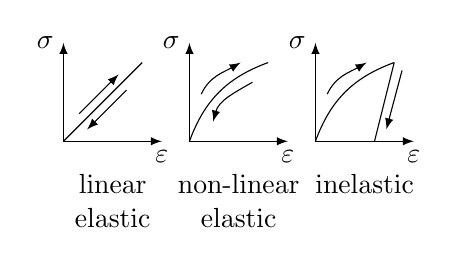
\begin{tikzpicture}[scale=0.5, >=latex]
    % --- Linear Elastic ---
    \begin{scope}[shift={(0,0)}]
        \draw[->] (0,0) -- (2.5,0) node[below] {$\varepsilon$};
        \draw[->] (0,0) -- (0,2.5) node[left] {$\sigma$};
        %\node[below left] at (0,0) {$O$};
        \draw (0,0) -- (2,2);
        \draw[->] (0.4, 0.7) -- (1.4, 1.7);
        \draw[->] (1.6, 1.3) -- (0.6, 0.3);
        \node[below, align=center] at (1.25, -0.6) {linear\\elastic};
    \end{scope}

    % --- Non-Linear Elastic ---
    \begin{scope}[shift={(3.2,0)}]
        \draw[->] (0,0) -- (2.5,0) node[below] {$\varepsilon$};
        \draw[->] (0,0) -- (0,2.5) node[left] {$\sigma$};
        %\node[below left] at (0,0) {$O$};
        \draw (0,0) to[out=70, in=200] (2,2);
        \draw[->] (0.3, 1.2) to[out=65, in=210] (1.3, 2.0);
        \draw[->] (1.6, 1.5) to[out=210, in=75] (0.6, 0.5);
        \node[below, align=center] at (1.25, -0.6) {non-linear\\elastic};
    \end{scope}

    % --- Inelastic ---
    \begin{scope}[shift={(6.4,0)}]
        \draw[->] (0,0) -- (2.5,0) node[below] {$\varepsilon$};
        \draw[->] (0,0) -- (0,2.5) node[left] {$\sigma$};
        %\node[below left] at (0,0) {$O$};
        \draw (0,0) to[out=70, in=200] (2,2);
        \draw (2,2) -- (1.5,0);
        \draw[->] (0.3, 1.2) to[out=65, in=210] (1.3, 2.0);
        \draw[->] (2.2, 1.8) -- (1.8, 0.3);
        \node[below, align=center] at (1.25, -0.6) {inelastic};
    \end{scope}
\end{tikzpicture}
\end{center}
Generalized Hooke's Law for linear elastic material: $\bm{\sigma} = \mathbb{C} : \bm{\varepsilon} \leftrightarrow \sigma_{ij} = C_{ijkl} \varepsilon_{kl}$.
\begin{itemize}
    \item \textbf{Elastic behavior:} 1) stress $\bm{\sigma}$ is a one-to-one function of strain $\bm{\varepsilon}$, 2) material returns to original configuration upon removal of forces.
    \item \textbf{Elasticity Tensor $\mathbb{C}$:} 4th-order, $3^4 = 81$ components.
    \item \textbf{Symmetries:}
        \subitem 1) \textit{Minor Symmetries:} $C_{ijkl} = C_{jikl}$ (due to $\bm{\sigma} = \bm{\sigma}^T$) and $C_{ijkl} = C_{ijlk}$ (due to $\bm{\varepsilon} = \bm{\varepsilon}^T$). $\implies$ 36 independent components.
        \subitem 2) \textit{Major Symmetry:} $C_{ijkl} = C_{klij}$ (if strain energy $U$ exists $\implies$ \textit{Hyperelastic}). $\implies$ \textbf{21 independent components}.
    \item \textbf{Internal Strain Energy Density $U$:} Energy per unit volume $[J/m^{3}]$.
        \subitem General Case: $U(\bm{\varepsilon}) = \frac{1}{2} C_{ijkl} \varepsilon_{ij} \varepsilon_{kl} = \frac{1}{2} \sigma_{ij} \varepsilon_{ij}$. 
        \subitem Isotropic Case: $U = \frac{1}{2} (\lambda \varepsilon_{kk} \varepsilon_{ii} + 2\mu \varepsilon_{ij} \varepsilon_{ij}) = $
        \subitem $ = \frac{1}{2E}((1+\nu)\sigma_{ij}\sigma_{ij}-\nu\sigma_{kk}\sigma_{ii}) = \frac{\lambda-2\mu}{2} I^{(\varepsilon)^2}_1 + 2\mu I_2^{(\varepsilon)}$.        
        \subitem Loading Scenarios:
            \subitem \textit{Uniaxial:} $I = \frac{\sigma_0^2}{2E}$
            \subitem \textit{Pure Shear:} $U = \frac{\tau_0^2}{2G}$
            \subitem \textit{Hydrostatic:} $U = \frac{p^2}{2K}$
        \subitem \textbf{Hyperelastic:} $\sigma_{ij} = \frac{\partial U}{\partial \varepsilon_{ij}}$ and $C_{ijkl} = \frac{\partial^2 U}{\partial \varepsilon_{ij} \partial \varepsilon_{kl}}$.
        \subitem \textbf{Stability:} $U(\bm{\varepsilon}) > 0$ for $\bm{\varepsilon} \neq \bm{0} \implies \mathbb{C}$ is positive definite. $E, G, K > 0$ required.
    \item \textbf{Material Properties:}
        \subitem \textit{Homogeneous:} $C_{ijkl}$ independent of position $\bm{x}$.
        \subitem \textit{Isotropic:} Material properties independent of direction.
\end{itemize}

\subsection{Isotropic Linear Elastic Solids}
Material properties independent of direction. Characterized by 2 constants ($\lambda, \mu$).

\textbf{Stress:} $ \boxed{\sigma_{ij} = \lambda \delta_{ij} \varepsilon_{kk} + 2\mu \varepsilon_{ij}} \quad \leftrightarrow \quad \bm{\sigma} = \lambda \text{tr}(\bm{\varepsilon})\bm{I} + 2\mu \bm{\varepsilon} $

Alternative Inverse Forms:
\[ \varepsilon_{ij} = \frac{1}{2\mu} \sigma_{ij} - \frac{\lambda}{2\mu} \varepsilon_{kk} \delta_{ij} = \frac{1}{2\mu} \sigma_{ij} - \frac{\lambda}{2\mu(3\lambda+2\mu)} \sigma_{kk} \delta_{ij} \]
Inverted form (Hooke's Law):
\[ \boxed{\varepsilon_{ij} = \frac{1}{E} [(1+\mu)\sigma_{ij} - \mu \delta_{ij} \sigma_{kk}]} \quad\leftrightarrow\quad \bm{\varepsilon} = \frac{1+\nu}{E} \bm{\sigma} - \frac{\nu}{E} \text{tr}(\bm{\sigma})\bm{I} \]
Material Constants and Relations:
\begin{itemize}
    \item $\lambda, \mu$: Lamé parameters. $G = \mu$ (Shear modulus).
    \item $E$: Young's Modulus. $E = \frac{\sigma}{\varepsilon} = \frac{F/A}{\Delta L/L_0} = \frac{\mu(3\lambda + 2\mu)}{\lambda + \mu} > 0$. $\uparrow E \rightarrow \uparrow \text{stiffness}$.
    \item $\nu$: Poisson's ratio. $\nu = \frac{\lambda}{2(\lambda+\mu)} = -\frac{\varepsilon_{lateral}}{\varepsilon_{axial}} \in [-1, 0.5]$. 
        \subitem $\nu = 0$: no lateral strain.
        \subitem $\nu = 0.5$: $K->\infty$ incompressible.
        \subitem $\nu < 0$: auxetic (material/structure gets thicker when pulling).
    \item $K$: Bulk modulus $K = \lambda + \frac{2}{3}\mu = \frac{E}{3(1-2\nu)} > 0$.
    \item $G$: Shear modulus $G = \frac{E}{2(1+\nu)} > 0, \quad \lambda = \frac{E\nu}{(1+\nu)(1-2\nu)}$.
\end{itemize}

\begin{center}

\small
\begin{tabular}{|p{1.3cm}|p{2.0cm}|l|p{0.6cm}|p{1.2cm}|}
    \hline
    \textbf{Property} & \textbf{Definition} & \textbf{Formula} &\textbf{Unit} & \textbf{Appl.} \\ \hline
    Bulk Mod. (K) & Resistance to uniform compression & $K = \frac{p}{\varepsilon_{kk}}=\frac{p}{\nicefrac{\Delta V}{V_0}}$ & Pa & Fluids, Pressure \\ \hline
    Shear Mod. (G=$\mu$) & Resistance to shear deformation & $G = \frac{\tau_{ij}}{2\varepsilon_{ij}}=\frac{\bm{\tau}}{\bm{\gamma}}$ & Pa & Torsion, Shear \\ \hline
    Young's Mod. (E) & Resistance to tensile/comp. loads & $E = \frac{\sigma}{\varepsilon}$ & Pa & Beams, Trusses \\ \hline
\end{tabular}
\end{center}

The stress $\sigma_{ij}$ consists of a 
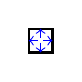
\begin{tikzpicture}[scale=0.3, baseline=0pt]
    \draw[thick] (0,0) rectangle (1,1);
    \foreach \x/\y/\r in {0.5/1/-90, 1/0.5/180, 0.5/0/90, 0/0.5/0}
        \draw[->, blue] (\x,\y) ++(\r:0.4) -- (\x,\y);
\end{tikzpicture}
\textit{hydrostatic} ($H_{ij} = \frac{1}{3} \sigma_{kk} \delta_{ij}$) and a
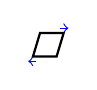
\begin{tikzpicture}[scale=0.3, baseline=0pt]
    \draw[thick] (0,0) -- (1,0) -- (1.3,1) -- (0.3,1) -- cycle;
    \draw[->, blue] (1.15,1.2) -- (1.5,1.2);
    \draw[->, blue] (0.15,-0.2) -- (-0.2,-0.2);
\end{tikzpicture}
\textit{deviatoric} ($S_{ij} = \sigma_{ij} - H_{ij} = \sigma_{ij} - \frac{1}{3} \sigma_{kk} \delta_{ij}$) part. 

\subsection{Formulation of Problems in Three-dimensional Linear Elasticity}
Governing equations for isotropic linear elastostatics:
\begin{enumerate}
    \item Equilibrium: $\sigma_{ij,j} + \rho b_i = 0$
    \item Kinematics: $\varepsilon_{ij} = \frac{1}{2}(u_{i,j} + u_{j,i})$
    \item Constitutive: $\sigma_{ij} = \lambda \varepsilon_{kk} \delta_{ij} + 2\mu \varepsilon_{ij} \\\text{or}\quad \varepsilon_{ij} = \frac{1}{E} [(1+\mu)\sigma_{ij} - \mu \delta_{ij} \sigma_{kk}]$
\end{enumerate}
\textbf{Navier's Equations} (Displacement formulation):
\[ \mu u_{i,jj} + (\lambda + \mu) u_{j,ij} + \rho b_i = 0 \]
Vector form:
\[ \mu \nabla^2 \bm{u} + (\lambda + \mu) \nabla (\nabla \cdot \bm{u}) + \rho \bm{b} = \bm{0} \]

\subsubsection*{Specific Problems}
\begin{itemize}
    \item \textbf{Uniaxial Extension (Bar):} $\sigma_{11} = \sigma_0$, others 0. \\By Constitutive: $\varepsilon_{11} = \sigma_0/E, \varepsilon_{22} = \varepsilon_{33} = -\nu \varepsilon_{11}$. \\
    \textit{Solution Verification:} 1) Equilibrium satisfied, 2) Boundary Conditions (BCs) met $\bm{t}=\bm{\sigma n} = BC's$, 3) Compatibility/Kinematics (integrability of strains to a valid displacement field $\bm{u}$).
    \item \textbf{Pure Bending:} Moment couple $\bm{M}$ at ends. Lateral surfaces traction-free, $\rho \bm{b} = \bm{0}$.
        \subitem Assumption: $\sigma_{11}$ only $\implies \frac{\partial \sigma_{11}}{\partial x_1}=0$, so $\sigma_{11}(x_2, x_3)$.
        \subitem Compatibility: $\frac{\partial^2 \sigma_{11}}{\partial x_k^2}=0$ ($k=2,3$)
        \subitem $\implies$ linear: $\sigma_{11} = \alpha + \beta x_2 + \gamma x_3$.
        \subitem Centroidal Axes: $\alpha = 0$. Principal Axes ($I_{23}=0$):
        \[ \sigma_{11} = -\frac{M_3}{I_{33}}x_2 + \frac{M_2}{I_{22}}x_3 \]
        \subitem Strain-Curvature: $\varepsilon_{11} = -y\kappa$ (implicitly $\sigma_{11}/E$). $\varepsilon_{22} = \varepsilon_{33} = -\nu \varepsilon_{11}$.
\end{itemize}

\section{Two-Dimensional Continua}

\subsection{Plane strain solutions}
Long body (along $x_3$), loading transverse.
Assumptions: $\varepsilon_{13} = \varepsilon_{23} = \varepsilon_{33} = 0$. $u_3 = 0$. Thus $\bm{u}, \bm{\sigma}, \bm{\varepsilon}$ are functions $f(x_1,x_2) \neq f(x_1,x_2,x_3)$. 
Stresses:
\[ \sigma_{33} = \nu(\sigma_{11} + \sigma_{22}) \neq 0 \]
In-plane relations same as 3D.

\subsection{Plane stress solutions}
Thin body (thickness $h$ along $x_3$), loading in-plane $(x_1, x_2)$.
Assumptions: $\sigma_{33} = \sigma_{13} = \sigma_{23} = 0$.
Strains:
\begin{align*}
    \varepsilon_{11} &= \frac{1}{E}(\sigma_{11} - \nu \sigma_{22}) \\
    \varepsilon_{22} &= \frac{1}{E}(\sigma_{22} - \nu \sigma_{11}) \\
    \varepsilon_{33} &= -\frac{\nu}{E}(\sigma_{11} + \sigma_{22})
\end{align*}
For isotropic, linear elastic material: $\varepsilon_{13}=\varepsilon_{23}=0, \varepsilon_{33}\neq 0$\\
Constitutive (Stress-Strain):
\[ \sigma_{ij} = \frac{E}{1-\nu^2} [(1-\nu)\varepsilon_{ij} + \nu \delta_{ij} \varepsilon_{kk}] \quad (i,j = 1,2) \]

\subsection{Airy Stress Function}
To satisfy equilibrium $\nabla \cdot \bm{\sigma} = \bm{0}$ in 2D, introduce scalar function $\phi(x_1, x_2)$, where compatibility requires $\phi$ to satisfy the \textbf{Biharmonic Equation} (if body forces are constant/zero):
\[ \nabla^4 \phi = \frac{\partial^4 \phi}{\partial x_1^4} + 2\frac{\partial^4 \phi}{\partial x_1^2 \partial x_2^2} + \frac{\partial^4 \phi}{\partial x_2^4} = 0 \]
equivalent to 
\begin{align*}
    \frac{\partial \sigma_{11}}{\partial x_{1}} + \frac{\partial \sigma_{12}}{\partial x_{2}} = 0, \quad \frac{\partial \sigma_{12}}{\partial x_{1}} + \frac{\partial \sigma_{22}}{\partial x_{2}} = 0, \quad \frac{\partial \sigma_{33}}{\partial x_{3}} = 0
\end{align*}
\textbf{Strains from Airy Stress Function:}
Using constitutive laws (Hooke's Law):
\begin{itemize}
    \item \textbf{Plane Stress:}
    \begin{align*}
        &\sigma_{11} = \frac{1}{E}\left(\frac{\partial^2 \phi}{\partial x_2^2} - \nu \frac{\partial^2 \phi}{\partial x_1^2}\right) = \frac{\partial^2 \phi}{\partial x_2^2} \\
        &\sigma_{22} = \frac{1}{E}\left(\frac{\partial^2 \phi}{\partial x_1^2} - \nu \frac{\partial^2 \phi}{\partial x_2^2}\right) = \frac{\partial^2 \phi}{\partial x_1^2} \\
        &\sigma_{12} = -\frac{1+\nu}{E} \frac{\partial^2 \phi}{\partial x_1 \partial x_2} = -\frac{\partial^2 \phi}{\partial x_1 \partial x_2}
    \end{align*}
    \item \textbf{Plane Strain:}
    \begin{align*}
        &\varepsilon_{11} = \frac{1+\nu}{E}\left((1-\nu)\frac{\partial^2 \phi}{\partial x_2^2} - \nu \frac{\partial^2 \phi}{\partial x_1^2}\right) = \frac{1}{E} (\sigma_{11} - \nu \sigma_{22}) \\
        &\varepsilon_{22} = \frac{1+\nu}{E}\left((1-\nu)\frac{\partial^2 \phi}{\partial x_1^2} - \nu \frac{\partial^2 \phi}{\partial x_2^2}\right) = \frac{1}{E} (\sigma_{22} - \nu \sigma_{11}) \\
        &\varepsilon_{12} = -\frac{1+\nu}{E} \frac{\partial^2 \phi}{\partial x_1 \partial x_2} = - \frac{\nu}{E} (\sigma_{11} + \sigma_{22}) \\
        &\varepsilon_{13} = \varepsilon_{23} = 0
    \end{align*}
    \item \textbf{Total external Forces at $x_1=L$:} 
    \subitem1) $\bm{t} = \bm{\sigma} \bm{n}$ ($\bm{n}$ normal vector, here $x_1$) 
    \subitem2) $\bm{F} = \int_A \bm{t}dA = \int_0^{thickness} \int_{min}^{max} \bm{t} dx_2dx_3$
\end{itemize}

\section{Truss}
One-dimensional element (bar) along $x_1$, cross-section $A(x_1)$.
Assumptions: $\sigma_{11}(x_1)$ is the only non-zero stress component.
Equilibrium Condition (with distributed load $\hat{b}_1 = \rho A b_1$):
\[ \frac{d}{dx_1}(A \sigma_{11}) + \hat{b}_1 = 0 \]
Constitutive: $\sigma_{11} = E \varepsilon_{11} = E \frac{du_1}{dx_1}$.
Governing Equation (Displacement):
\[ \frac{d}{dx_1}\left( E A \frac{du_1}{dx_1} \right) + \hat{b}_1 = 0 \]
For constant $E, A$: $E A u_1'' + \hat{b}_1 = 0$.

\section{Selected Problems}

\subsection{Problem 1: Tensors \& Eigenvalues}
\textbf{Problem Statement:}
\begin{enumerate}
    \item Given that tensors $\mathbf{R}$ and $\mathbf{S}$ have the same eigenvector $\mathbf{n}$ and corresponding eigenvalues $r$ and $s$, respectively, find an eigenvalue and the corresponding eigenvector for $\mathbf{T} = \mathbf{RS}$.
    \item Find the value of the expression $\delta_{1i}\delta_{ij}\delta_{j2}$.
\end{enumerate}

\textbf{Solution:}
\begin{enumerate}
    \item We have $\mathbf{Rn} = r\mathbf{n}$ and $\mathbf{Sn} = s\mathbf{n}$.
    
    Applying $\mathbf{T}$ to $\mathbf{n}$:
    \[ \mathbf{Tn} = \mathbf{RSn} = \mathbf{R}(s\mathbf{n}) = s(\mathbf{Rn}) = s(r\mathbf{n}) = rs\mathbf{n} \]
    
    Thus, an eigenvalue for $\mathbf{T} = \mathbf{RS}$ is $rs$ with eigenvector $\mathbf{n}$.

    \item Using the substitution property of the Kronecker delta:
    \[ \delta_{1i}\delta_{ij}\delta_{j2} = \delta_{1i} (\delta_{i2}) = \delta_{12} = 0 \]
\end{enumerate}

\subsection{Problem 2: Divergence Theorem}
\textbf{Problem Statement:}
Verify that $\int_B \nabla \cdot \mathbf{F} \, dV = \int_{\partial B} \mathbf{F} \cdot \mathbf{n} \, dS$ where $B$ is the cylinder defined by $x_1^2 + x_2^2 \leq 1, 0 \leq x_3 \leq 1$.
$\mathbf{F}$ is given by components $F_i = x_3 \delta_{i3}$ (i.e., $\mathbf{F} = [0, 0, x_3]^T$).

\textbf{Solution:}
\textbf{Left Hand Side (Volume Integral):}
\[ \nabla \cdot \mathbf{F} = F_{i,i} = \frac{\partial (x_3 \delta_{i3})}{\partial x_i} = \frac{\partial x_3}{\partial x_3} = 1 \]
\[ \int_B \nabla \cdot \mathbf{F} \, dV = \int_B 1 \, dV = \text{Volume of Cylinder} = (\pi r^2) h = \pi(1)^2(1) = \pi \]

\textbf{Right Hand Side (Surface Integral):}
Boundary $\partial B$ consists of three parts:
\begin{itemize}
    \item $S^{(1)}$ (Lateral surface, $x_1^2+x_2^2=1$): $\mathbf{n}^{(1)} = [x_1, x_2, 0]^T$. $\mathbf{F} = [0, 0, x_3]^T$.
    \[ \mathbf{F} \cdot \mathbf{n}^{(1)} = 0 \implies \int_{S^{(1)}} \mathbf{F} \cdot \mathbf{n} \, dS = 0 \]
    
    \item $S^{(2)}$ (Top surface, $x_3=1$): $\mathbf{n}^{(2)} = [0, 0, 1]^T$. $\mathbf{F} = [0, 0, 1]^T$.
    \[ \int_{S^{(2)}} \mathbf{F} \cdot \mathbf{n}^{(2)} \, dS = \int_{S^{(2)}} 1 \, dS = \text{Area} = \pi \]
    
    \item $S^{(3)}$ (Bottom surface, $x_3=0$): $\mathbf{n}^{(3)} = [0, 0, -1]^T$. $\mathbf{F} = [0, 0, 0]^T$.
    \[ \int_{S^{(3)}} 0 \, dS = 0 \]
\end{itemize}
Total Surface Integral = $0 + \pi + 0 = \pi$.
The theorem is verified.

\subsection{Problem 3: Plane Strain Beams/Dams}
\textbf{Problem Statement:}
A prismatic dam with triangular cross-section has boundaries:
\begin{itemize}
    \item Face BC (Vertical): Normal $\mathbf{n} = [0, 1, 0]^T$, no traction.
    \item Face OB (Base): Normal $\mathbf{n} = [-1, 0, 0]^T$ ?, traction due to water/gravity? (See assumptions below).
    \item Face AC (Sloped): Normal $\mathbf{n} = [1, 0, 0]^T$, no traction.
\end{itemize}
Assume displacement field:
\[ u_1 = -4x^2 - y^2 + 2xy + 2, \quad u_2 = -4y^2 - x^2 + 2xy + 5 \]
Material: $E=100$ MPa, $\nu=0.4$, Plane Strain. Find the stress field.

\textbf{Solution:}
\textbf{1. Calculate Strains:}
\[ \varepsilon_{11} = \frac{\partial u_1}{\partial x} = -8x + 2y \]
\[ \varepsilon_{22} = \frac{\partial u_2}{\partial y} = -8y + 2x \]
\[ \gamma_{12} = 2\varepsilon_{12} = \frac{\partial u_1}{\partial y} + \frac{\partial u_2}{\partial x} = (2x - 2y) + (2y - 2x) = 0 \]

\textbf{2. Calculate Stresses (Plane Strain):}
Using Hooke's Law for Plane Strain:
\[ \sigma_{11} = \frac{E}{(1+\nu)(1-2\nu)} [(1-\nu)\varepsilon_{11} + \nu\varepsilon_{22}] \]
\[ \sigma_{22} = \frac{E}{(1+\nu)(1-2\nu)} [\nu\varepsilon_{11} + (1-\nu)\varepsilon_{22}] \]
\[ \sigma_{12} = G \gamma_{12} = \frac{E}{2(1+\nu)} \cdot 0 = 0 \]

Substituting values ($C = \frac{100}{1.4 \cdot 0.2} = 357.14$ MPa):
\[ \sigma_{11} = 357.14 [0.6(-8x+2y) + 0.4(-8y+2x)] = 357.14 [-4x - 2y] \]
\[ \sigma_{22} = 357.14 [0.4(-8x+2y) + 0.6(-8y+2x)] = 357.14 [-2x - 4y] \]
\[ \sigma_{33} = \nu(\sigma_{11} + \sigma_{22}) = 0.4(\sigma_{11} + \sigma_{22}) \]

\subsection{Problem 4: Airy Stress Function - Beam (Sample)}
\textbf{Problem Statement:}
A cantilever beam (fixed at $x_1=a$, force $F$ at $x_1=0$) has Airy stress function within Plane Stress ($\delta=1$):
\[ \Phi = \frac{F}{4b^3} (x_1 x_2^3 - 3b^2 x_1 x_2) \]
Verify validity and calculate stresses.

\textbf{Solution:}
\textbf{1. Validity (Biharmonic Equation):}
$\nabla^4 \Phi = 0$?
\[ \frac{\partial^4 \Phi}{\partial x_1^4} = 0, \quad \frac{\partial^4 \Phi}{\partial x_2^4} = 0, \quad \frac{\partial^4 \Phi}{\partial x_1^2 \partial x_2^2} = 0 \]
Sum = 0. valid.

\textbf{2. Stresses:}
\[ \sigma_{11} = \frac{\partial^2 \Phi}{\partial x_2^2} = \frac{F}{4b^3} (6x_1 x_2) = \frac{3F}{2b^3} x_1 x_2 \]
\[ \sigma_{22} = \frac{\partial^2 \Phi}{\partial x_1^2} = 0 \]
\[ \sigma_{12} = -\frac{\partial^2 \Phi}{\partial x_1 \partial x_2} = -\frac{F}{4b^3} (3x_2^2 - 3b^2) = \frac{3F}{4b^3} (b^2 - x_2^2) \]

\textbf{3. Reaction Forces at $x_1=a$:}
Shear Force: $\int_{-b}^{b} \sigma_{12}(a, x_2) dx_2 = F$.
Moment: $-\int_{-b}^{b} \sigma_{11}(a, x_2) x_2 dx_2 = -Fa$.

\subsection{Problem 5: Airy Stress Function - Mars Rover Solar Panel}
\textbf{Problem Statement:}
The stresses in the solar panel of a Mars rover can be approximated by an Airy stress function:
\[ \Phi = a_1 x_1^2 + a_2 x_1 x_2 + a_3 x_2^2 \]

\textbf{a) Verify that it satisfies the biharmonic equation.}
\[ \nabla^4 \Phi = \frac{\partial^4 \Phi}{\partial x_1^4} + 2\frac{\partial^4 \Phi}{\partial x_1^2 \partial x_2^2} + \frac{\partial^4 \Phi}{\partial x_2^4} = 0 + 0 + 0 = 0 \]
Satisfied as the fourth order derivatives are 0.

\textbf{b) Determine the in-plane stresses $\sigma_{11}, \sigma_{12}, \sigma_{22}$.}
\[ \sigma_{11} = \frac{\partial^2 \Phi}{\partial x_2^2} = 2a_3, \quad \sigma_{22} = \frac{\partial^2 \Phi}{\partial x_1^2} = 2a_1, \quad \sigma_{12} = -\frac{\partial^2 \Phi}{\partial x_1 \partial x_2} = -a_2 \]

\textbf{c) Determine and sketch the reactions on the four rectangular boundaries ($x_1=0, x_1=b, x_2=0, x_2=c$).}

\begin{figure}[h]
\begin{center}
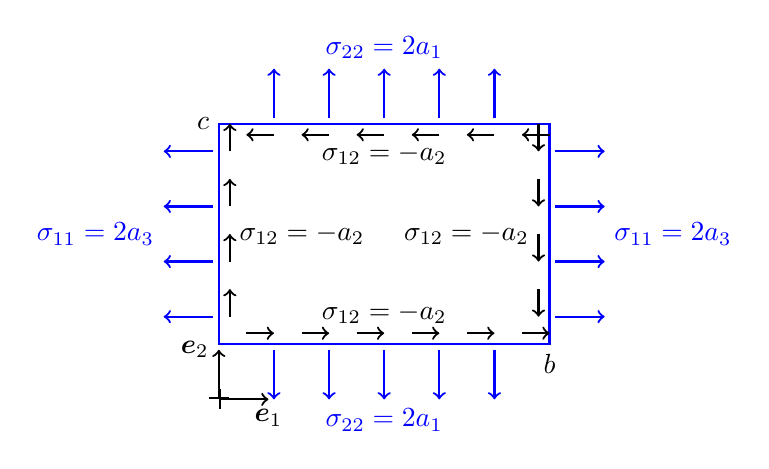
\begin{tikzpicture}[scale=0.7]
    % Coordinate System
    \draw[thick, |->] (0,-1) -- (0.9,-1) node[below] {$\bm{e}_1$};
    \draw[thick, |->] (0,-1) -- (0,-0.1) node[left] {$\bm{e}_2$};

    % Plate dimensions
    \draw[thick, blue] (0,0) rectangle (6,4);
    
    % Normal Stresses Sigma_11 (X-Direction) = 2a3
    \foreach \y in {0.5, 1.5, 2.5, 3.5} {
        \draw[thick, blue, <-] (-1, \y) -- (-0.1, \y); % Left
        \draw[thick, blue, ->] (6.1, \y) -- (7, \y);   % Right
    }
    \node[blue, left] at (-1, 2) {$\sigma_{11}=2a_3$};
    \node[blue, right] at (7, 2) {$\sigma_{11}=2a_3$};

    % Normal Stresses Sigma_22 (Y-Direction) = 2a1
    \foreach \x in {1, 2, 3, 4, 5} {
        \draw[thick, blue, ->] (\x, 4.1) -- (\x, 5);   % Top
        \draw[thick, blue, ->] (\x, -0.1) -- (\x, -1); % Bottom
    }
    \node[blue, above] at (3, 5) {$\sigma_{22}=2a_1$};
    \node[blue, below] at (3, -1) {$\sigma_{22}=2a_1$};

    % Shear Stresses (Sigma 12 = -a2). 
    % On positive x1 face (n=e1), t_2 = sigma_21 = -a2 (downwards)
    % On positive x2 face (n=e2), t_1 = sigma_12 = -a2 (leftwards)
    
    % Top Edge (n=e2). Traction t = sigma * n = [-a2, 2a1]. Shear component is -a2 e1 (Left)
    \foreach \x in {5.5, 4.5, ..., 0.5} {
        \draw[thick, black, ->] (\x+0.5, 3.8) -- (\x, 3.8);
    }
    \node[black, below] at (3, 3.8) {$\sigma_{12}=-a_2$};
    
    % Right Edge (n=e1). Traction t = [2a3, -a2]. Shear component is -a2 e2 (Down)
    \foreach \y in {3.5, 2.5, ..., 0.5} {
        \draw[thick, black, ->] (5.8, \y+0.5) -- (5.8, \y);
    }
    \node[black, left] at (5.8, 2) {$\sigma_{12}=-a_2$};

    % Bottom Edge (n=-e2). Traction t = -[-a2, 2a1] = [a2, -2a1]. Shear is a2 e1 (Right)
    \foreach \x in {0.5, 1.5, ..., 5.5} {
        \draw[thick, black, ->] (\x, 0.2) -- (\x+0.5, 0.2);
    }
    \node[black, above] at (3, 0.2) {$\sigma_{12}=-a_2$};

    % Left Edge (n=-e1). Traction t = -[2a3, -a2] = [-2a3, a2]. Shear is a2 e2 (Up)
     \foreach \y in {0.5, 1.5, ..., 3.5} {
        \draw[thick, black, ->] (0.2, \y) -- (0.2, \y+0.5);
    }
    \node[black, right] at (0.2, 2) {$\sigma_{12}=-a_2$};
    
    % Labels b and c
    \node[below] at (6,0) {$b$};
    \node[left] at (0,4) {$c$};

\end{tikzpicture}
    
Normal arrows point outward (reversed if minus). \\
Shear arrows point in $\bm{e}_j$ direction (reversed if minus). 
\end{center}
\end{figure}



Boundary Tractions $\bm{t} = \bm{\sigma} \cdot \bm{n}$:
\begin{itemize}
    \item $x_1 = 0, \bm{n} = -\bm{e}_1$: $\bm{t} = - (2a_3 \bm{e}_1 - a_2 \bm{e}_2) = -2a_3 \bm{e}_1 + a_2 \bm{e}_2$.
    \item $x_1 = b, \bm{n} = \bm{e}_1$: $\bm{t} = 2a_3 \bm{e}_1 - a_2 \bm{e}_2$.
    \item $x_2 = 0, \bm{n} = -\bm{e}_2$: $\bm{t} = - (-a_2 \bm{e}_1 + 2a_1 \bm{e}_2) = a_2 \bm{e}_1 - 2a_1 \bm{e}_2$.
    \item $x_2 = c, \bm{n} = \bm{e}_2$: $\bm{t} = -a_2 \bm{e}_1 + 2a_1 \bm{e}_2$.
\end{itemize}

\textbf{d) As a plane strain solution, determine $\sigma_{13}, \sigma_{23}, \sigma_{33}$ and strains.}
Plane strain ($\varepsilon_{13}=\varepsilon_{23}=\varepsilon_{33}=0$). Isotropic material.
\[ \sigma_{33} = \nu(\sigma_{11} + \sigma_{22}) = \nu(2a_3 + 2a_1), \quad \sigma_{13} = \sigma_{23} = 0 \]
Strains (using Hooke's Law with $\sigma_{33}$ substituted):
\begin{align*}
    \varepsilon_{11} &= \frac{1}{E}[(1-\nu^2)2a_3 - \nu(1+\nu)2a_1] \\
    \varepsilon_{22} &= \frac{1}{E}[(1-\nu^2)2a_1 - \nu(1+\nu)2a_3] \\
    \varepsilon_{12} &= -\frac{1+\nu}{E} a_2 \\
    \varepsilon_{13} &= \varepsilon_{23} = \varepsilon_{33} = 0
\end{align*}

\textbf{e) As a plane stress solution, determine $\sigma_{13}, \sigma_{23}, \sigma_{33}$ and strains.}
Plane stress by definition ($\sigma_{13}=\sigma_{23}=\sigma_{33}=0$):
\begin{align*}
    \varepsilon_{11} &= \frac{1}{E}(2a_3 - 2\nu a_1) \\
    \varepsilon_{22} &= \frac{1}{E}(2a_1 - 2\nu a_3) \\
    \varepsilon_{12} &= -\frac{1+\nu}{E} a_2 \\
    \varepsilon_{33} &= -\frac{\nu}{E}(2a_3 + 2a_1), \quad \varepsilon_{13} = \varepsilon_{23} = 0
\end{align*}



\subsection{Problem 6: Airy Stress Function - Dam}
\textbf{Problem Statement:}
A dam approximated as an isotropic, elastic block $ABC$ under plane strain.
\begin{itemize}
    \item Airy Stress Function: $\Phi(x, y) = \frac{1}{6}a_1 x^3 + \frac{1}{2}a_2 x^2 y + \frac{1}{2}a_3 x y^2 + \frac{1}{6}a_4 y^3$
    \item Boundary $AB$ ($x=0$): Hydrostatic pressure $p = \rho g y$.
    \item Boundary $AC$: Free surface.
\end{itemize}

\textbf{a) Determine stress components and constants.}

\textbf{1. Biharmonic Equation:}
$\nabla^4 \Phi = 0$ is satisfied (4th derivatives of cubic polynomial are 0).

\textbf{2. Stress Components:}
\[ \sigma_{11} = \frac{\partial^2 \Phi}{\partial y^2} = a_3 x + a_4 y \]
\[ \sigma_{22} = \frac{\partial^2 \Phi}{\partial x^2} = a_1 x + a_2 y \]
\[ \sigma_{12} = -\frac{\partial^2 \Phi}{\partial x \partial y} = -(a_2 x + a_3 y) \]
Plane Strain: $\sigma_{33} = \nu(\sigma_{11} + \sigma_{22})$.

\textbf{3. Boundary Conditions:}
\begin{itemize}
    \item \textbf{Along AB ($x=0$):} Normal $\bm{n} = -\bm{e}_1$. Traction $\bm{t} = p \bm{e}_1 = \rho g y \bm{e}_1$.
    \[ \bm{t} = \bm{\sigma} \bm{n} = -\sigma_{11}(0,y)\bm{e}_1 - \sigma_{12}(0,y)\bm{e}_2 = -a_4 y \bm{e}_1 + a_3 y \bm{e}_2 \]
    Matching components:
    \[ -a_4 y = \rho g y \implies a_4 = -\rho g \]
    \[ a_3 y = 0 \implies a_3 = 0 \]

    \item \textbf{Along AC:} Normal $\bm{n} = \frac{1}{\sqrt{2}}(\bm{e}_1 - \bm{e}_2)$ (Slope $x=y$). Traction $\bm{t} = \bm{0}$.
    \[ \bm{t} = \bm{\sigma} \bm{n} = \frac{1}{\sqrt{2}} \begin{pmatrix} \sigma_{11} - \sigma_{12} \\ \sigma_{12} - \sigma_{22} \end{pmatrix}_{x=y} = \bm{0} \]
    Substitute $a_3=0, a_4=-\rho g$:
    \[ \sigma_{11} - \sigma_{12} = (-\rho g y) - (-a_2 x) = (a_2-\rho g)x = 0 \implies a_2 = \rho g \]
    \[ \sigma_{12} - \sigma_{22} = (-a_2 x) - (a_1 x + a_2 y) = -(2a_2 + a_1)x = 0 \implies a_1 = -2a_2 = -2\rho g \]
\end{itemize}
\textbf{Resulting Constants:}
$a_1 = -2\rho g, \quad a_2 = \rho g, \quad a_3 = 0, \quad a_4 = -\rho g$.

\textbf{b) Tractions on BC for equilibrium.}
Along BC ($y=l$), Normal $\bm{n} = \bm{e}_2$.
Traction vector $\bm{t}$:
\[ \bm{t} = \bm{\sigma} \bm{n} = \sigma_{12}(x,l)\bm{e}_1 + \sigma_{22}(x,l)\bm{e}_2 \]
Substituting constants:
\[ \sigma_{12} = -(\rho g x + 0) = -\rho g x \]
\[ \sigma_{22} = -2\rho g x + \rho g l = \rho g (l - 2x) \]
\[ \implies \bm{t}|_{BC} = -\rho g x \bm{e}_1 + \rho g (l - 2x) \bm{e}_2 \]

\begin{center}
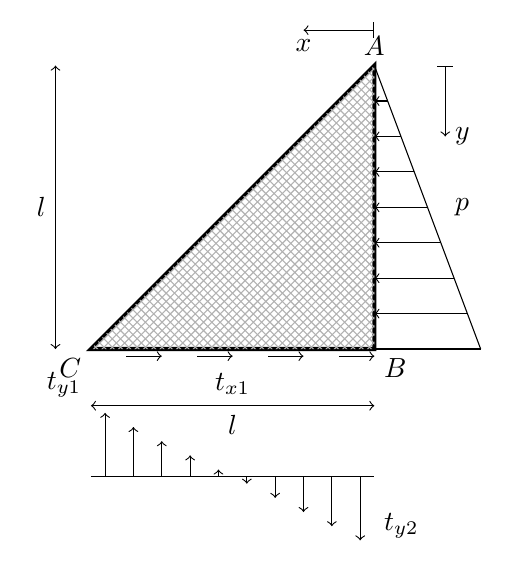
\begin{tikzpicture}[scale=0.9]
    % Coordinates matching the visual representation
    % A (Top Right), B (Bottom Right), C (Bottom Left)
    \coordinate (A) at (4,4); 
    \coordinate (B) at (4,0); 
    \coordinate (C) at (0,0); 
    
    % Draw Triangle (Dam)
    \draw[line width=1.5pt] (A) -- (B) -- (C) -- cycle;
    
    % Hatching pattern for the dam body
    \fill[pattern=crosshatch, pattern color=black!30] (A) -- (B) -- (C) -- cycle;
    
    % Labels for vertices
    \node[above] at (A) {$A$};
    \node[below right] at (B) {$B$};
    \node[below left] at (C) {$C$};
    
    % Axes (Origin at A approx, x left, y down)
    \draw[|->] (4, 4.5) -- (3, 4.5) node[below] {$x$};
    \draw[|->] (5, 4) -- (5, 3) node[right] {$y$};
    
    % Dimensions
    \draw[<->] (-0.5, 0) -- (-0.5, 4) node[midway, left] {$l$}; % Vertical Height
    \draw[<->] (0, -0.8) -- (4, -0.8) node[midway, below] {$l$}; % Horizontal Width

    % Hydrostatic Pressure p on AB (Right vertical face)
    % Triangular distribution, increasing downwards
    \draw (4,4) -- (5.5,0); % Slope line of pressure
    \draw (4,0) -- (5.5,0); % Bottom line
    \foreach \y in {0.5, 1.0, 1.5, 2.0, 2.5, 3.0, 3.5} {
        % Arrows pointing Left onto the surface
        \draw[->] ({4 + (4-\y)*1.5/4}, \y) -- (4, \y);
    }
    \node[right] at (5, 2) {$p$};
    
    % Tractions on BC (Bottom horizontal face)
    % 1. Shear stress tx1 (Horizontal arrows pointing Right)
    \foreach \x in {0.5, 1.5, 2.5, 3.5} {
        \draw[->] (\x, -0.1) -- (\x+0.5, -0.1);
    }
    \node[below] at (2, -0.2) {$t_{x1}$};
    
    % 2. Normal stress ty1/ty2 (Vertical and distributed)
    % We want a linear distribution from Upward on the left (C) to Downward on the right (B).
    % The base of the dam is from x=0 (C) to x=4 (B) in TikZ coordinates.
    % The traction arrows should be drawn relative to a baseline below the dam.
    \draw (0,-1.8) -- (4,-1.8); % Baseline for the stress distribution

    % Loop for arrows
    \foreach \x in {0.2, 0.6, ..., 4.0} {
        % Calculate height: Linear function f(x)
        % Let's say at x=0 height is +1.0 (Up), at x=4 height is -1.0 (Down)
        % h = 1.0 - 0.5*x
         \pgfmathsetmacro{\h}{1.0 - 0.5*\x}
         \draw[->] (\x, -1.8) -- (\x, {-1.8 + \h});
    }

    % Labels
    \node[left] at (0, -0.5) {$t_{y1}$};
    \node[right] at (4, -2.5) {$t_{y2}$};

\end{tikzpicture}
\end{center}

\end{document}
